\chapter{Historische Grundlage} %TODO Titel ändern? --> Grundlagen
\section{Implementierungsformen von Software}
Um Programme in einer bestimmten Programmiersprache für einen \ac{PC} lesbar zu machen müssen diese in Maschinencode, quasi die Muttersprache des \ac{PC}'s, übersetzt werden \cite[vgl. Wagenknecht Hielscher 2022, S.2ff]{wagenknecht_hielscher_2022}. Dazu gibt es verschiedene technische Implementierungsformen, die folgend kurz vorgestellt werden:

\subsection{Compiler}\label{ch_compiler}
Der Compiliervorgang ist ähnlich einem Übersetzungsvorgang von z.B. einem chinesischen Text in englische Sprache zu  sehen und kann gerade bei größeren Programmen durchaus Zeit in Anspruch nehmen und der Quellcode muss für jede Änderung erneut compiliert werden. Als Vorteil ist jedoch die schnelle Ausführung durch das Zielsystem zu nennen, da der Programmcode komplett in die korrespondierende Instruktionen dieses Zielsystems übersetzt wurde. \cite[vgl. Wagenknecht Hielscher, S.121]{wagenknecht_hielscher_2022}
Andererseits muss das Zielsystem bereits beim Compilationsvorgang bekannt sein und es kann nur allgemein für ein System, aber nicht zwangsläufig für die tatsächlich darunter liegende Hardware übersetzt werden. \\
Durch den Einsatz von höheren Programmiersprachen wurde der Einsatz von Compilern nötig, um den verfassten Quellcode für die jeweiligen Zielsysteme in den geeigneten Maschinencode zu übersetzen. Die für den Menschen einfacher zu verstehenden Programmiersprachen (auch Hochsprachen) bieten die Möglichkeit ihre Logik für verschiedene Zielsysteme durch einen Compiler zu übersetzen und somit sowohl dem Menschen, als auch dem \ac{PC} ein gut lesbares Format vorzuhalten, \cite[vgl. Wagenknecht Hielscher, S.1ff]{wagenknecht_hielscher_2022}.\\
Bereits Konrad Zuse setzte für seinen Zuse Z4 auf eine Art höhere Sprache, das sogenannte Plankalkül und wollte mit einem 'Planfertigungsgerät' automatisch von einem mathematischen Rechenplan einen Lochstreifen mit gestanztem Maschinenplan anfertigen, \cite[vgl. Heilige 2013, S.45]{Hellige2013}. Nach heutiger Terminologie ist dieses Planfertigungsgerät bereits als Compiler zu betrachten. \\
Der erste Compiler A-0 wurde von Grace Hopper 1952 vorgestellt und erleichterte den Prozess der Programmierung hinlänglich, da statt direkter Maschinenbefehle nun Code aus verständlichen Algorithmen, die in einem Katalog zusammengefasst waren, aufgebaut werden konnten. Diese Bausteine wurden von A-0 aus dem Katalog abgerufen und der Code in korrekter Reihenfolge zusammen gesetzt. Benötigte Speicherbereiche wurden automatisch reserviert und die zugehörige Adressierung ebenfalls vom Compiler übernommen, \cite[vgl. Beyer 2012, S.222ff]{Beyer2012}. In der Weiterentwicklung, dem Prototypen B-0 konnten Befehle in verschiedenen menschlichen Sprachen (z.B. Englisch, Französisch, Deutsch) verwendet werden, die der Computer zu Maschinencode übersetzte, \cite[vg. Beyer 2012, S.271ff]{Beyer2012}.\\
Über Compiler für die Sprachen Fortran und COBOL wurden die Compiler schlussendlich soweit entwickelt, wie wir sie heute kennen. 

\subsection{Interpreter} \label{ch_interpreter}
Da die Klasse der Interpreter nicht konkret Teil dieser Arbeit, aber mit den Themen eng verwandt ist, soll hier kurz auf den Aufbau und die Geschichte eingegangen werden. \\
Ein Interpreter führt portionsweise Aktionen aus und interpretiert so zur Laufzeit den Quellcode zu maschinenlesbaren Instruktionen, wobei er im Unterschied zum Compiler keinen neuen Text erzeugt, sondern direkt den Quellcode zu Anweisungen übersetzt, \cite[vgl. Wagenknecht Hielscher 2022, S.4]{wagenknecht_hielscher_2022}. Interpreter werden oft von Skriptsprachen eingesetzt und ersparen den Compilationsvorgang im Vorfeld. \\
Außerdem können Interpretersprachen plattformunabhängig ausgeliefert werden, da die Interpretation erst auf dem Zielsystem ausgeführt wird und im Vorfeld nicht bekannt sein muss, auf welchem \ac{OS} der Quellcode ausgeführt werden soll. Das Zielsystem kann den Code somit für sich selbst interpretiere und die Instruktionen somit auch direkt für die eigene Hardware zielgerichtet umsetzen. \\
Andererseits entsteht durch die Interpretation zur Laufzeit ein erhöhter Aufwand, der Interpretersprachen grundsätzlich eine langsamere Ausführung beschert, als im Vorfeld zu Maschinencode kompilierten Programmen.\\
Interpreter entstanden ungefähr zur selben Zeit, wie die ersten Compiler und wurden erfunden, um zwischen verschiedenen Low-level-Sprache zu übersetzen und die allgemeine Programmierung zu vereinfachen, \cite[vgl. Bennet 1952, S.81 f]{Bennett1952}. \\
Der erste Interpreter wurde dabei von John Russel zusammen der Sprache LISP auf einem IBM 704 entwickelt, der dazu diente Lisp-Programme zu evaluieren, \cite[vgl. Stoyan S.299ff]{Stoyan1984}

\subsection{Just-in-time-Kompilierung} \label{ch_jit}
Die Implementierungsform der \ac{JIT}-Kompilierung versucht die Vorteile von \autoref{ch_interpreter} und \autoref{ch_compiler} zu vereinen. Einerseits wird der Code vorab zu Bytecode kompiliert, um eine schnellere Ausführung in einer \ac{VM} zu ermöglichen, andererseits wird der Code zur Laufzeit direkt auf der Zielmaschine von Bytecode in Maschinencode kompiliert, was den Vorteil bietet, dass dieser speziell für den ausführenden Prozessor optimiert werden kann.\\
\ac{JIT} vereint damit den Vorteil der Plattformunabhängigkeit des Interpreters mit dem Geschwindigkeitsvorteil des Compilers. Die Vorteile können dabei nicht genauso stark ausgespielt werden, wie bei den ursprünglichen Implementierungsformen, aber es wird ein sehr guter Mittelweg geschaffen, um sich die Leistung moderner Rechner zunutze zu machen und direkt auf dem Zielsystem zu compilieren, um die Geschwindigkeit des ausgeführten Programmteils maßgeblich zu erhöhen, als auch die Auslieferung von direkt übersetzbaren Bytecode, der die Software plattformunabhängig macht.\\
Die Anfänge des Gedanken der \ac{JIT}-Kompilierung reichen zurück bis in die 1960er Jahre, aber erst in den 1980er Jahren wurde durch Peter Deutsch und Allan Schiffmann eine Publikation basierend auf der Entwicklung mit der Sprache Smalltalk-80. Smalltalk ist eine objektorientierte Sprache, die in einer \ac{VM} (siehe \autoref{jit_vm}) ausgeführt wird und kommt damit dem Prinzip der \ac{JIT}-Kompilierung sehr nahe. Deutsch und Schiffmann beschleunigten die Ausführungszeit von Smalltalk-Code auf einem Mikroprozessor mit geringer Leistung durch Konvertierung des Codes in verschiedene Varianten, z.B. v-Code (virtuell) und n-Code (nativ), um so eine bestmögliche Performance bei begrenzter Hardware zu erreichen, \cite[vgl. Deutsch und Schiffmann 1984, S.1ff]{Deutsch_Schiffmann1984}.\\
Für die Sprache Java wurden einige Aspekte aus Smalltalk-80 abgeleitet, wie zum Beispiel der Einsatz der \ac{VM}. 1999 wurde hierfür die \ac{VM} 'HotSpot' entwickelt, die einen \ac{JIT}-Compiler enthält. Anhand von heuristischen Methoden werden hier Codeblöcke, die oft ausgeführt werden ('Hot Spots'), kompiliert und somit die Ausführung von Programmen beschleunigt \cite[vgl. Kotzmann und Wimmer 2008, S.2ff]{KotzmannWimmer2008}

% TODO: Profildaten --> Was wird compiliert und warum --> Heuristik

\section{Programmausführung in der VM} \label{jit_vm}
Durch die Dynamik einer Programmiersprache, zur Schaffung einer Plattformunabhängigkeit oder aus Sicherheitsgründen werden Programme heutzutage oftmals nicht mehr direkt vom Betriebssystem ausgeführt, sondern laufen in einer \ac{VM}, wie dies bereits bei Smaltalk-80 der Fall war. Dies verzögert jedoch die Ausführungszeit der Interpretation der Befehle. \\
Durch die Anwendung von \ac{JIT} wird hier versucht Performance zu gewinnen und somit diesen Nachteil auszugleichen. Folgend sollen die beiden \ac{VM}'s 'HotSpot' und 'Graal' aus dem Kontext der Sprache Java näher vorgestellt werden. 
\subsection{HotSpot}
Java übersetzt den Code der Hochsprache generell zuerst in Bytecode, der in der \ac{VM} ausgeführt werden kann. Diese \ac{VM} wird speziell für das korrespondierende \ac{OS} bereitgestellt und kann auf dieser Plattform den erzeugten Bytecode korrekt ausführen. 'HotSpot' von Oracle ist eine dieser \ac{VM}'s für die Sprache Java. \\
\\
\begin{figure}[ht]
    \begin{center}
        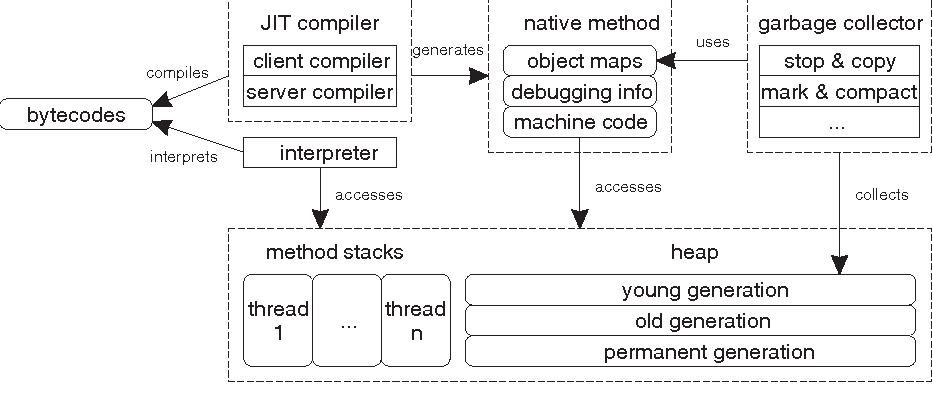
\includegraphics[width=0.9\textwidth]{assets/img/3-Figure1-1.png}
        \caption{Architektur 'HotSpot', \cite[Quelle: Kotzmann Wimmer 2008]{KotzmannWimmer2008}}
        \label{arch_hotspot}
    \end{center}
\end{figure}
Wie in \autoref{arch_hotspot} zu sehen, beginnt die Ausführung in der 'HotSpot'-\ac{VM} beim Interpreter. Hier wird der Bytecode schrittweise ausgeführt anhand von Templates ausgeführt. Nur die heuristisch am meisten frequentierten Codeblöcke werden durch den \ac{JIT}-Compiler kompiliert.\\
Wird während der Ausführung eine besonders aufwändige Schleife entdeckt, so wird diese ebenfalls kompiliert und die Ausführung dafür gestoppt. Die Schwierigkeit besteht hierbei darin, dass die Ausführung zwischen Interpreter und dem kompilierten Code synchronisiert werden muss. Dafür wird ein neuer Stackframe erstellt und initialisiert. Die Ausführung der Methode geht im nativen Code weiter. Dieses Verfahren nennt man \ac{OSR}.\\
'HotSpot' enthält zwei verschiedene Compiler, die für Server- und Clientsysteme gedacht sind. Bei Serversystemen wird sehr großer Wert auf eine sehr gute Optimierung gelegt, dafür jedoch eine längere Kompilierungszeit in Kauf genommen. Für dauerhaft laufende Serveranwendungen geht man davon aus, dass bereits während der Anlaufphase der Software der \ac{JIT}-Compiler alle wichtigen Methoden und Blöcke kompiliert und optimiert. Die längere Zeit ist hierfür nicht relevant, da die einmal kompilierten Sequenzen danach während der ganzen Laufzeit der Software zu Verfügung stehen.\\
Der Compiler für die Clientsysteme zielt auf Programme mit \ac{GUI} ab. Hier wird der Fokus auf die Antwortzeit der Oberfläche und damit den Punkt \ac{UX} gelegt. Dazu ist der \ac{JIT}-Compiler auf eine schnelle Kompilierung statt Performance ausgelegt, \cite[vgl. Kotzmann und Wimmer 2008, S.3]{KotzmannWimmer2008}.\\

\subsection{Graal}

